\documentclass[12pt, a4paper]{article}

\usepackage{graphicx} % Для работы
\graphicspath{{img/}} % с картинками

\usepackage{enumitem} % Для нумерации списков
\usepackage{pifont}
\usepackage{fancyhdr}
\usepackage{array}
\usepackage[rightcaption]{sidecap} % Подпись рисунка была справа
\usepackage{caption} % Убрать Рис. 1:
\usepackage[a4paper, left=1.5cm, right=1.5cm, top=1.5cm, bottom=1.5cm]{geometry}
\usepackage{multicol}  %  несколько колонок
\usepackage{cmap} % поиск в PDF
\usepackage[T2A]{fontenc} % кодировка
\usepackage[utf8]{inputenc} % кодировка исходного текста
\usepackage[english,russian]{babel} % локализация и переносы
\usepackage{amsmath}

% Устанавливаем стиль страницы fancy
\pagestyle{fancy}
% Очищениe всех текущих настроек заголовков и нижних колонтитулов
\fancyhf{}
% Для установления в правой части нижнего колонтитула номер страницы
\fancyfoot[R]{\thepage}
% Для установления в левой части нижнего колонтитула
\fancyfoot[L]{3*}

\begin{document}

\thispagestyle{empty}
\begin{center}
    \textbf{\footnotesize Министерство науки и высшего образования Российской Федерации}

    \vspace{1em}
    {\tiny ФЕДЕРАЛЬНОЕ ГОСУДАРСТВЕННОЕ АВТОНОМНОЕ ОБРАЗОВАТЕЛЬНОЕ УЧРЕЖДЕНИЕ ВЫСШЕГО ОБРАЗОВАНИЯ}

    \vspace{1em}
    \textbf{\large «НАЦИОНАЛЬНЫЙ ИССЛЕДОВАТЕЛЬСКИЙ УНИВЕРСИТЕТ ИТМО»}

    \vspace{2em}
    \textbf{Факультет ПИиКТ}

    \vspace{2em}
    \textbf{Дисциплина: Информатика}

    \vspace{16em}
    
    {\Large \textit{\textbf{Лабораторная работа № 6}}}\\[1em]
    {\Large \textbf{Работа с системой компьютерной вёрстки \TeX}}\\[3em]
    Вариант: \textbf{90}
\end{center}

\vspace{10em}

\begin{flushright}
    Выполнил: Михайлов Петр Сергеевич \\
    Группа: P3111 \\
    Преподаватель: доцент, кандидат технических наук \\
    Малышева Татьяна Алексеевна
\end{flushright}
\vspace{6em}

\begin{center}
Санкт-Петербург, 2024
\end{center}
\setcounter{page}{66} % номер страницы
\begin{minipage}[10cm]{\textwidth}
    \setlength\columnsep{20pt}
    \setlength\parindent{24pt}
    \begin{multicols*}{2}
	 \hspace*{16pt} % неразрывный отступ
    10 к л а с с
    
    \begin{enumerate}[itemindent=32pt] % отступ для каждого элемента списка
      \setlength{\itemsep}{0pt}
      \setlength{\parskip}{0pt}
      \setcounter{enumi}{4} % начинаем с пяти
      
      \item См. задачу № 5 для 8-го класса.
      \item Докажите, что для любого тетраэдара существуют такие две плоскости, что отношение площадей проекций тетраэдра на эти плоскости не меньше $ \sqrt{2} $.
      \item Рассмотрим $n$ чисел $a_1, a_2, \dots, a_n$.
      Положим
    \[b_k = \frac{a_i + \dots + a_k}{k}  (\textrm{для } k = 1, 2, \dots) ,\] % выравнивание по центру+с новой строки 
    \[C = (a_1 - b_1)^2 + (a_2 - b_2)^2  + \dots + (a_n - b_n)^2,\] 
    \[D = (a_1 - b_n)^2 + (a_2 - b_n)^2  + \dots + (a_n - b_n)^2. \]
    
    Докажите неравенства $ C \le D \le 2C $.
    
    \item Рассмотрим последовательность чисел $ x_n = (1 + \sqrt{2} + \sqrt{3})^n $.  Каждое из них приводится к виду
    \[ x_n = q_n + r_n\sqrt{2} + s_n\sqrt{3} + t_n\sqrt{6},\]
    где $q_n, r_n, s_n, t_n$ --- целые числа. Найдите пределы
    \[ \lim_{n\to\infty} \frac{r_n}{q_n},\quad \lim_{n\to\infty} \frac{s_n}{q_n}, \quad \lim_{n\to\infty} \frac{t_n}{q_n}. \]
    
    \item См. задачу № 8 для 9-го класса.
    \end{enumerate}
    
    Как участники соревнования справились с этими задачами, видно из приведенной таблицы. К сожалению, некоторые задачи оказались довольно трудными. Так, у восьмиклассников с задачей № 2 справились только
\\
\null\hfill Т а б л и ц а 
\\
        \begin{tabular}{c|l|}
            \hline
            \rotatebox{90}{Результаты} & \multicolumn{1}{c}{Номера задач} \\
            \hline
             \rotatebox{270}{$+$ \rotatebox{90}{$\pm$} \rotatebox{90}{$\mp$}} &
                \begin{tabular}{cccccccccccc}
                     \multicolumn{12}{c}{\textbf{8 класс}} \\
                     1&2&3&4a&4б&5а&5б&5в&6&7а&7б&8 \\
                     \hline
                     15&2&1&26&2&24&17&4&7&4&2&4 \\
                     8&0&0&5&9&0&3&12&0&1&1&1 \\
                     2&0&0&0&5&0&2&4&1&1&2&2 \\
                \end{tabular} \\
             \rotatebox{270}{$+$ \rotatebox{90}{$\pm$} \rotatebox{90}{$\mp$}} & \begin{tabular}{ccccccccc}
                     \multicolumn{9}{c}{\textbf{9 класс}} \\
                     1&2&3а&3б&4&5&6&7&8 \\
                     \hline
                     44&9&17&2&0&23&23&9&6 \\
                     13&0&2&2&0&14&1&1&0 \\
                     0&1&1&3&5&11&1&4&1 \\
                \end{tabular} \\
            \rotatebox{270}{$+$ \rotatebox{90}{$\pm$} \rotatebox{90}{$\mp$}} & \begin{tabular}{ccccccccccc}
                     \multicolumn{11}{c}{\textbf{10 класс}} \\
                     1&2&3а&3б&3в&4&5&6&7&8&9 \\
                     \hline
                     42&12&29&11&1&1&23&5&6&11&2\\
                     2&4&2&3&2&0&11&1&2&7&0 \\
                     0&2&4&9&1&17&2&5&4&9&0 \\
                \end{tabular} \\
        \end{tabular}
\\
\\
два школьника, с задачей № 3 --- один школьник и с задачей № 8 --- четыре школьника. 
    
Никто из девятиклассников не решил задачи № 4 и только два человека полностью решили задачу № 3б.
    
Среди десятиклассников задачи № 3в и 4 полностью решили толь-
    \end{multicols*}
\end{minipage}

\begin{SCfigure}[][h] % h = here
	\caption*{\textbf{Восьмиклассники, награжденные Дипломами 1 степени (слева направо): Ю. Ткаченко, А. Балинский, А. Разборов, А. Боричев.}} % Звездочка для того, чтобы убрать Рис. 1:
	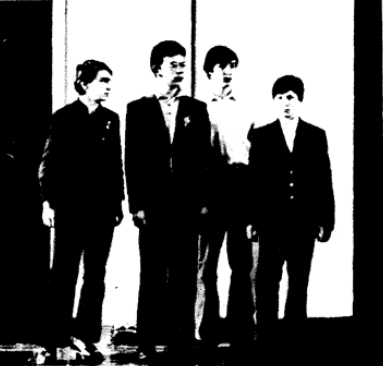
\includegraphics[scale=1]{8klass.png}
\end{SCfigure}

\end{document}